\chapter{Alternative Fit}
\label{chap:Appendix:AlternativeFit}

\FloatBarrier


While the final fit strategy for this thesis is presented in Section~\ref{sec:ChaptH:Fit},
alternative approaches are studied as well.  This approaches vary regarding how
the regions are defined


\section{Other \dilepOStau fits}

\subsection{Free float $k_{\ttbar}$ and $k_{\Zjets}$ and use dedicated CRs}
The mismodelling in some of the distributions at PR
is due to the wrong scale factors accounting for misidentification rates.
By letting $k_{\ttbar}$ and $k_{\Zjets}$ float as free parameters on the \dilepOStau, 
this can be fixed. To do so, the regions of the phase space enriched with such
processes enter in the fit as CRs (in contrast to the initial approach of use them as VRs).


\begin{figure}[h]
\centering
\begin{subfigure}{.3\textwidth}
  \centering
  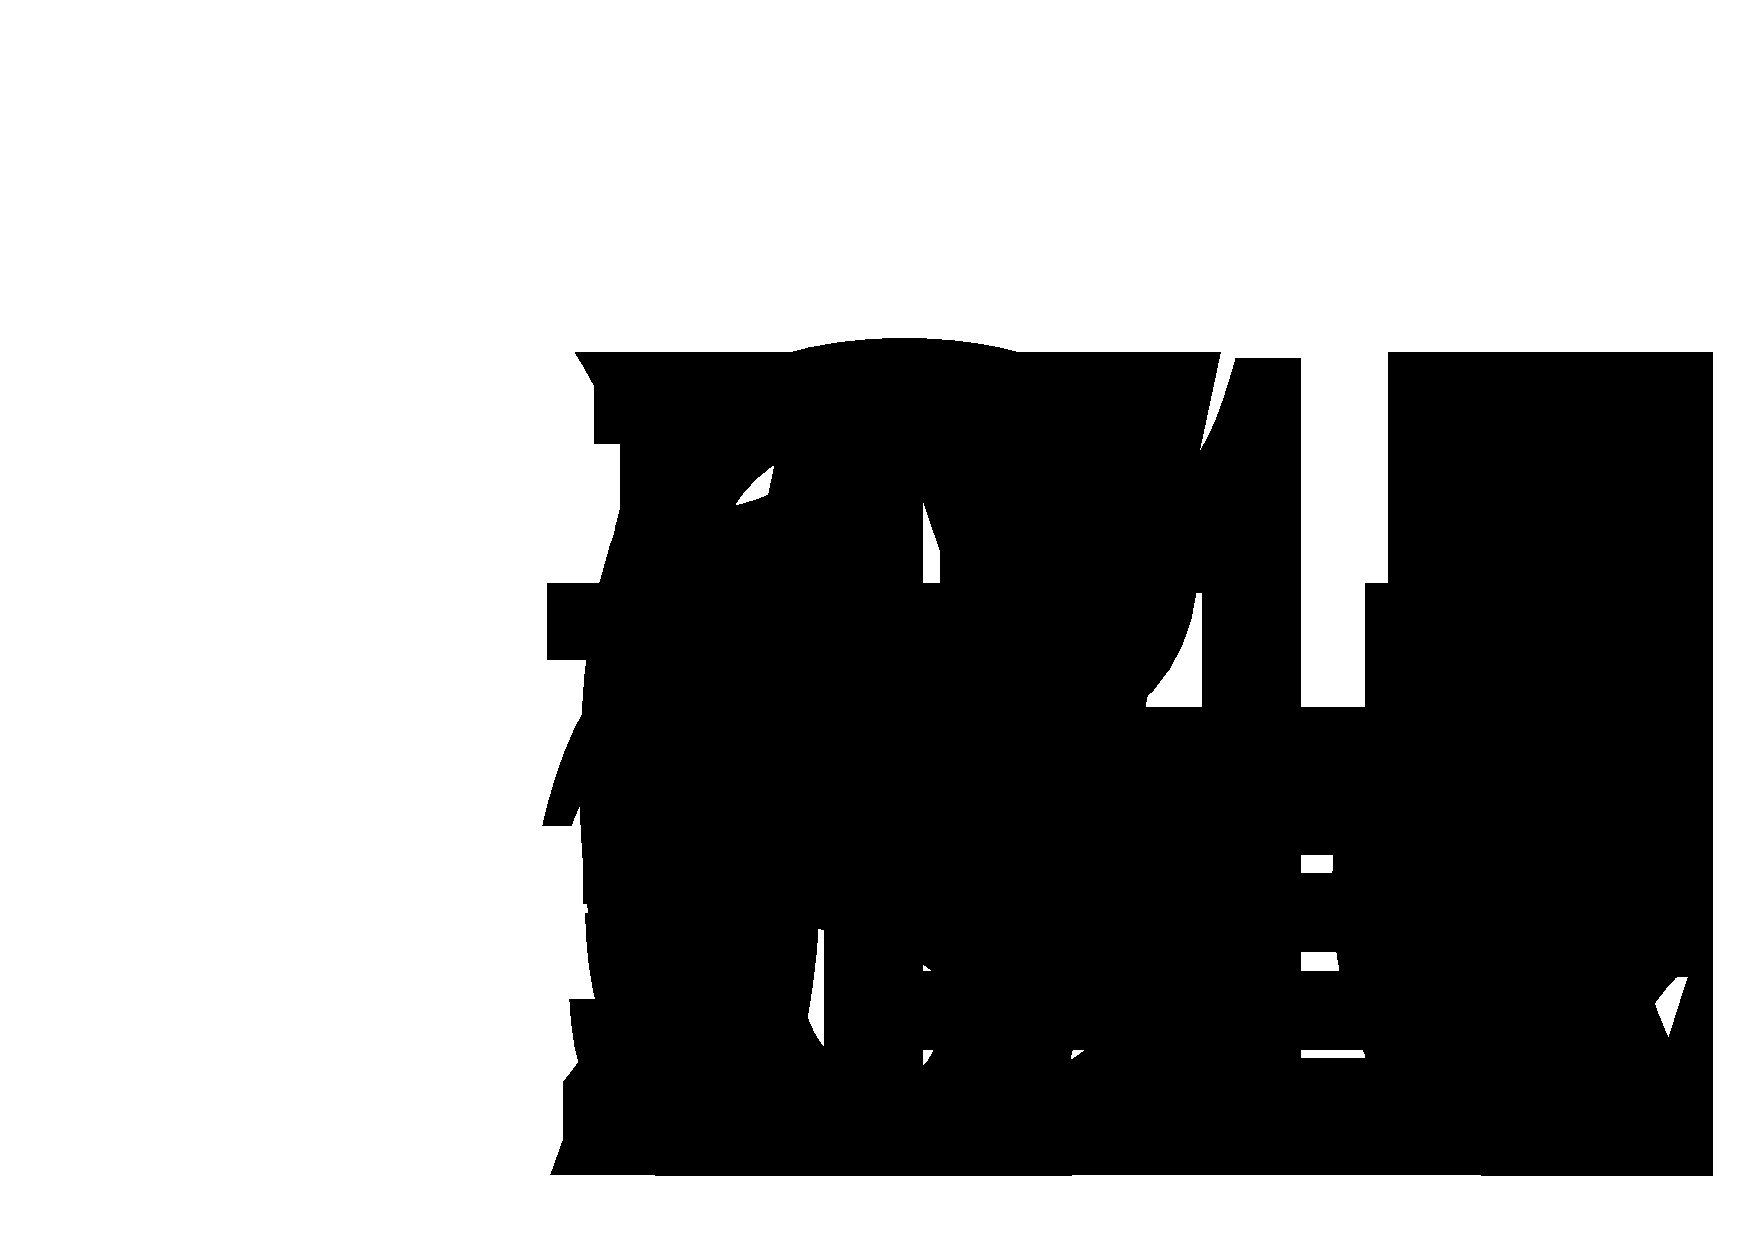
\includegraphics[width=.95\linewidth]{Chapter5_tHq/Alternative_Fit_Models/OS_Asimov_FreeFloat_K/SR_BDT_tHq_2L1TAU_OS}
  \caption{SR(\tHq)}
\end{subfigure}%
\begin{subfigure}{.3\textwidth}
  \centering
  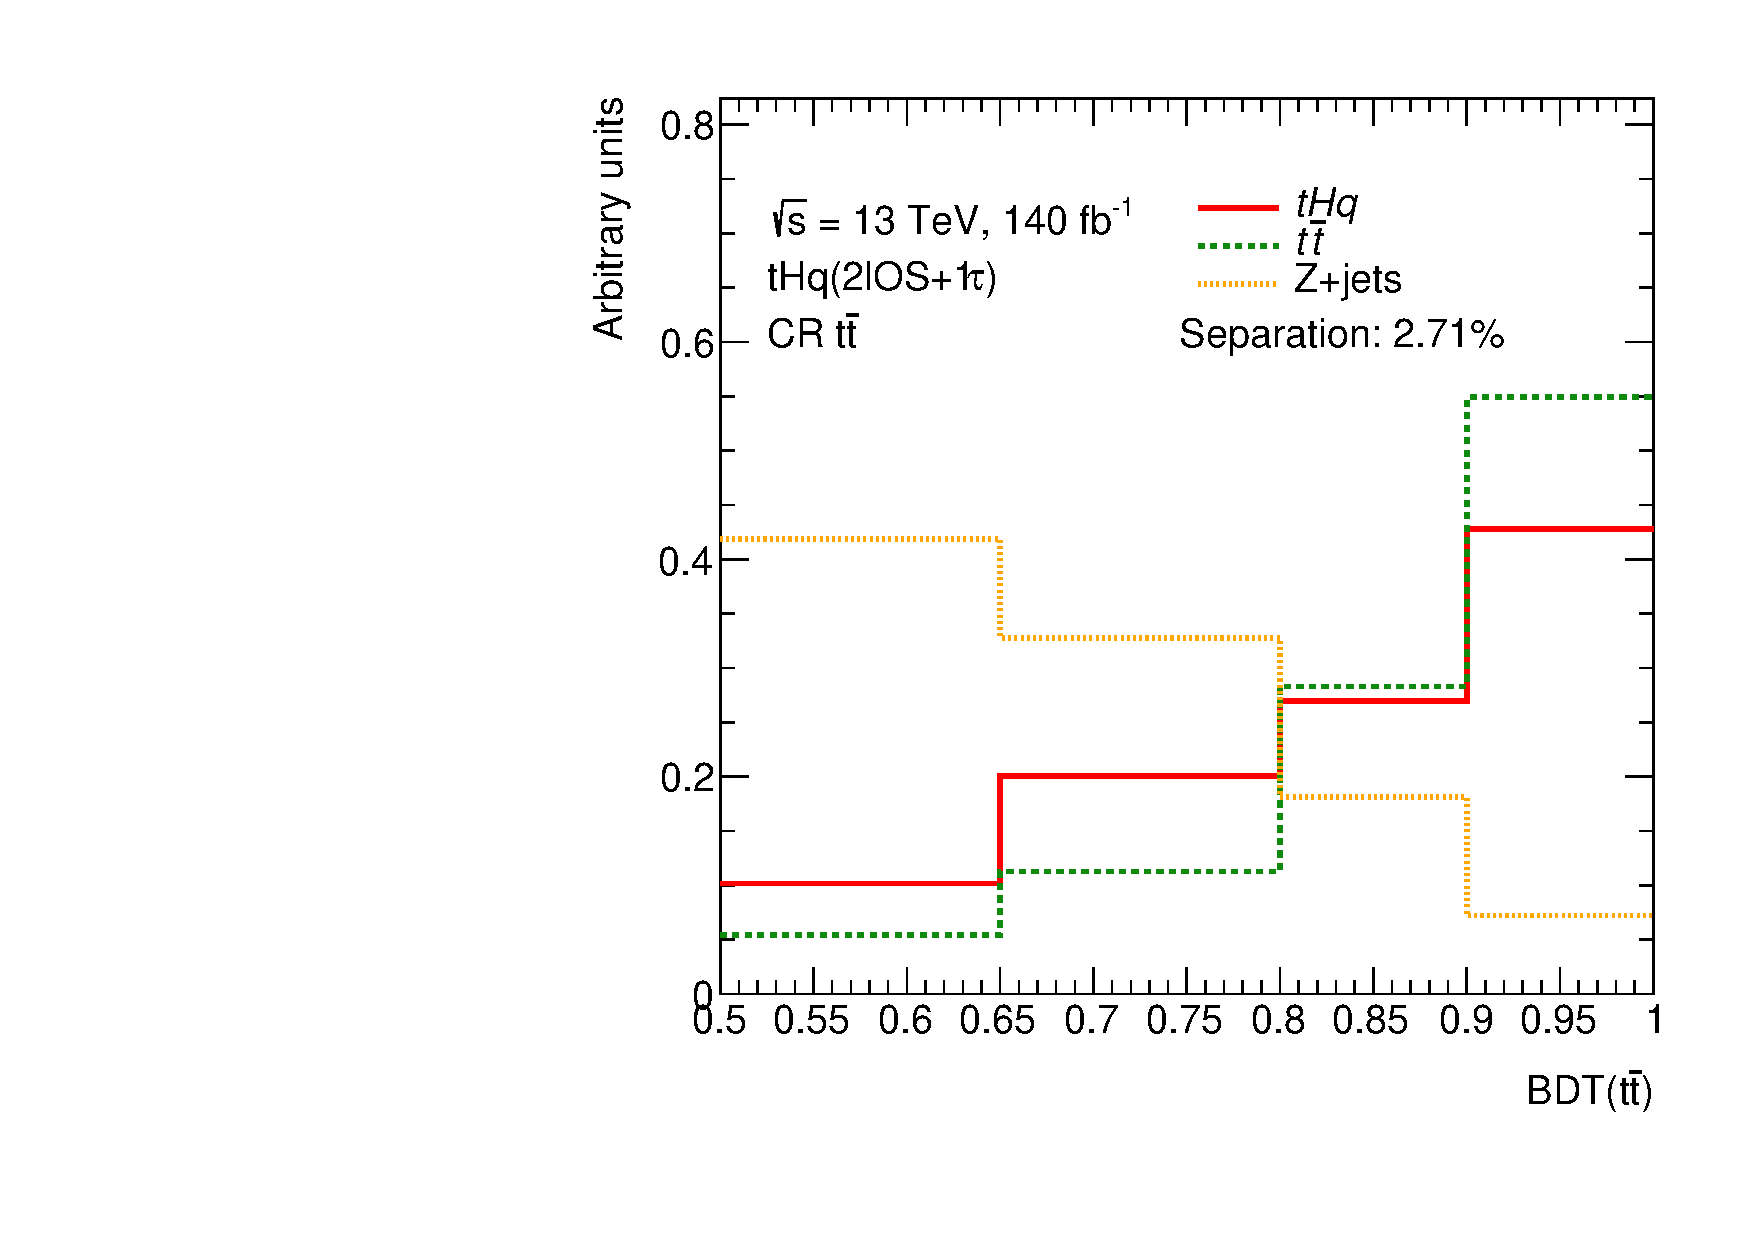
\includegraphics[width=.95\linewidth]{Chapter5_tHq/Alternative_Fit_Models/OS_Asimov_FreeFloat_K/CR_ttbar_2L1TAU_OS}
  \caption{CR(\ttbar)}
\end{subfigure}
\begin{subfigure}{.3\textwidth}
  \centering
  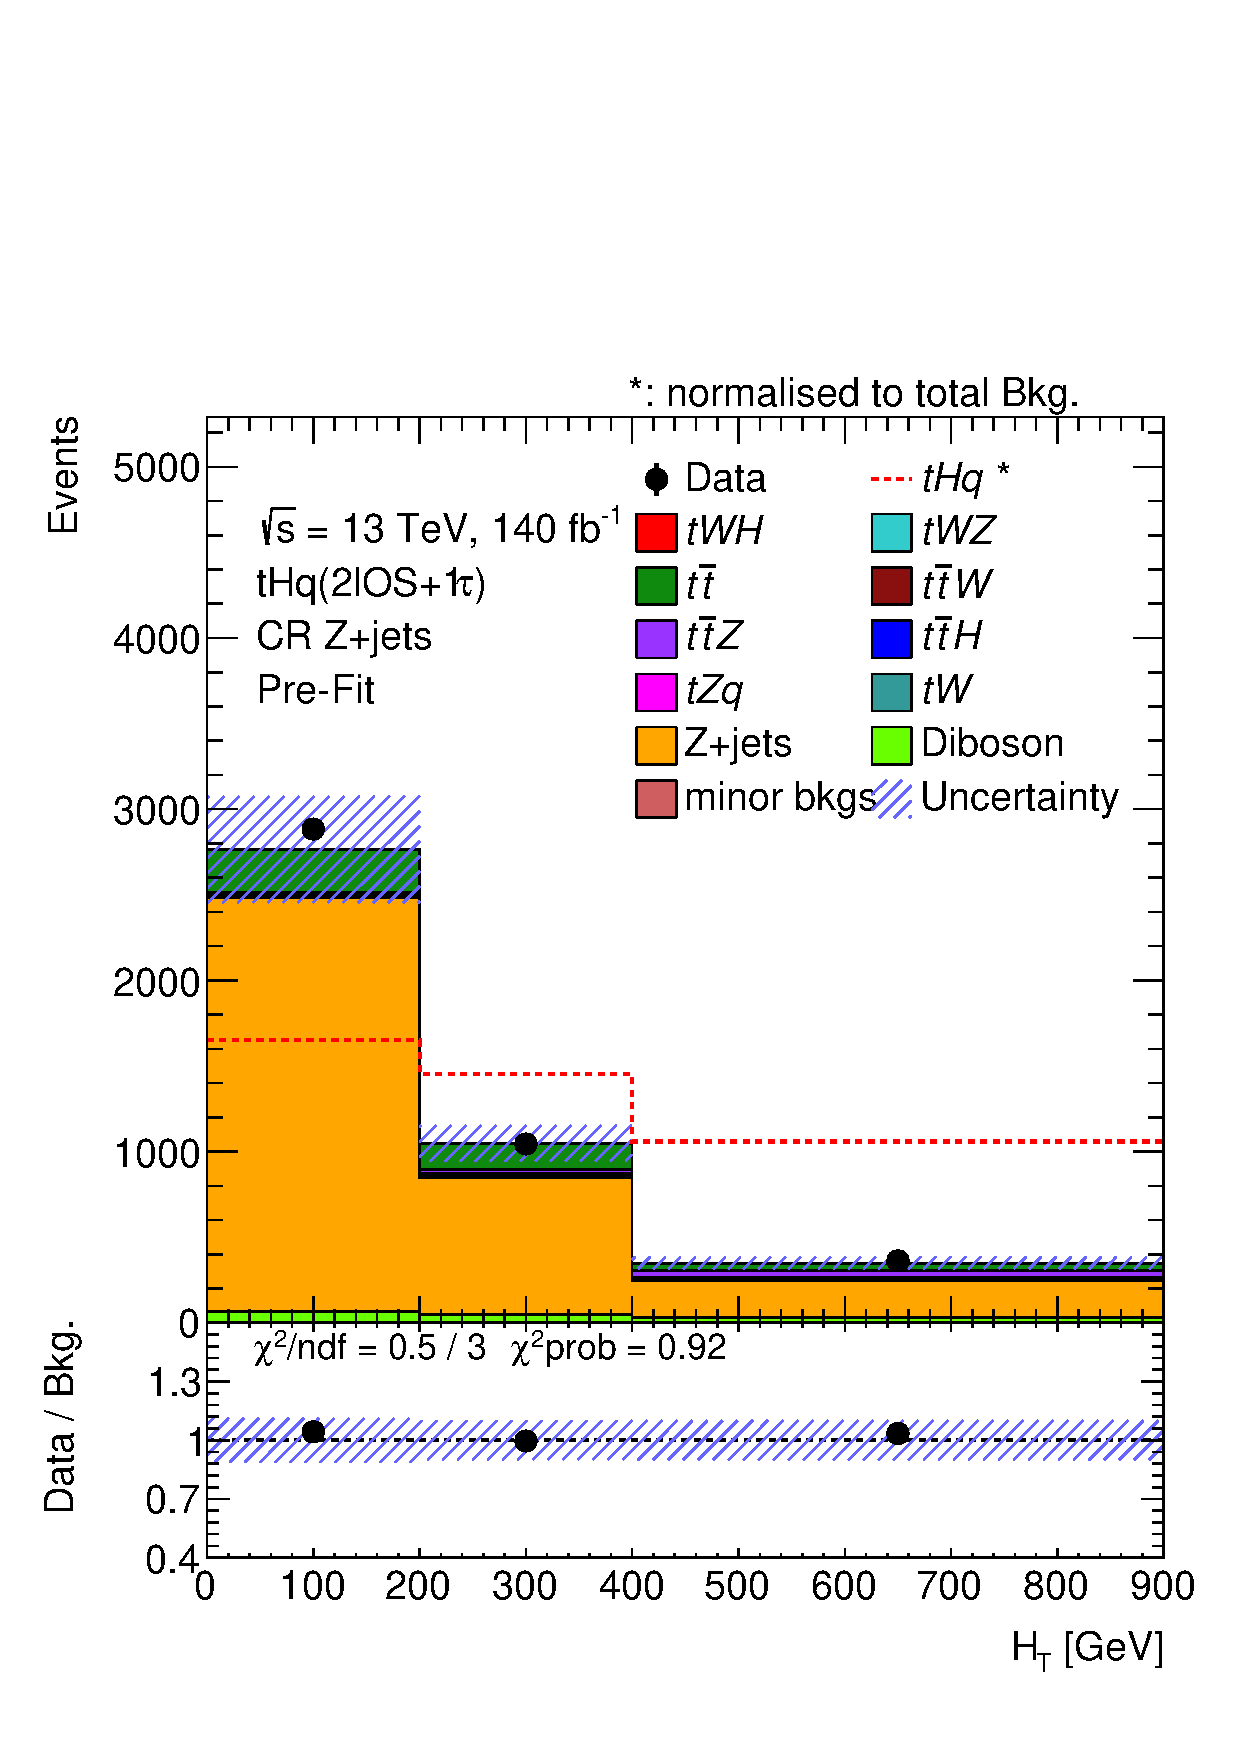
\includegraphics[width=.95\linewidth]{Chapter5_tHq/Alternative_Fit_Models/OS_Asimov_FreeFloat_K/CR_Zjets_2L1TAU_OS}
  \caption{CR(\Zjets)}
\end{subfigure}
\caption{Pre-fit distributions used for the \dilepOStau fit}
\label{fig:Alternative:PreFit:OS:VRs}
\end{figure}

When the normalisation factors are let to float, we get:
\begin{align*}
	\Delta \mu_{\tHq}^{\dilepOStau} (\text{expected})   &= \pm 17.09 (\text{tot.}) \pm 12.60 (\text{stat.}) \\
	\Delta \mu_{\ttbar}^{\dilepOStau} (\text{expected})  &= \pm 0.06 (\text{tot.}) \pm 0.02 (\text{stat.}) \\
	\Delta \mu_{\Zjets}^{\dilepOStau} (\text{expected}) &= \pm 0.11 (\text{tot.}) \pm 0.02 (\text{stat.}) \\
\end{align*}
In contrast, if these are fixed and no CRs are used in the fit:
\begin{align*}
	\Delta \mu_{\tHq}^{\dilepOStau} (\text{expected})   &= \pm 17.41  (\text{tot.}) \pm 12.44 (\text{stat.}) 
\end{align*}


At 95\% CL the expected limit is:
\begin{align*}
	\mu_{\tHq}^{\dilepOStau, \text{95CL}} (\text{expected})   &= 46.1^{+29.5}_{-16.4}
\end{align*}


\begin{figure}[h]
\centering
 \includegraphics[width=.95\linewidth]{Chapter5_tHq/Alternative_Fit_Models/OS_Asimov_FreeFloat_K/CorrMatrix}
\caption{Correlation in the \dilepOStau under the Asimov hypothesis when $k_{\ttbar}$ and $k_{\Zjets}$ are free parameters of the fit.} 
\label{fig:Other:Asimov:OS:Correlation}
\end{figure}
 

\begin{figure}[h]
\centering
\begin{subfigure}{.5\textwidth}
  \centering
  \includegraphics[width=.95\linewidth]{Chapter5_tHq/Alternative_Fit_Models/OS_Asimov_FreeFloat_K/Ranking_tH_NORM}
  \caption{Free floating $k_{\ttbar}$ and $k_{\Zjets}$ as well as $\mu_{\tHq}$}
\end{subfigure}%
\begin{subfigure}{.5\textwidth}
  \centering
  \includegraphics[width=.95\linewidth]{Chapter5_tHq/Alternative_Fit_Models/OS_Asimov_DoNotFreeFloat_K/Ranking_tH_NORM}
  \caption{Only $\mu_{\tHq}$ is a free floating parameter}
\end{subfigure}
\caption{Ranking plots in the \dilepOStau under the Asimov hypothesis.}
\label{fig:Alternative:PreFit:OS:Rankings}
\end{figure}



\section{Other \dilepSStau fits}

\subsection{Two regions only and floating $k_{\ttW}$}
\label{sec:Alternative:SS:OneCR_kttW}
In this configuration only the SR and single CR are used in the fit. 
The CR used here consists in all the events that do not enter the SR.
It is defined as:
\begin{itemize}
	\item SR(\tHq) :: BDT$(\tHq|_{\text{SS}}) \leq 0.4$ and fitting the BDT$(\tHq|_{\text{SS}})$ distribution.
	\item CR(all bkgs) :: BDT$(\tHq|_{\text{SS}}) > 0.4$ and fitting $H_{\text{T}}$ distributions. 
\end{itemize}
The normalisation factor for \ttW is let as a free-floating parameter of the fit. The distributions of the fit
are presented in Figure~\ref{fig:Alternative:SS:OneCR_kttW:distributions}. In these distributions is 
important to note the large discrepancy between the real data and MC-simulated samples.

\begin{figure}[h]
\centering
\begin{subfigure}{.5\textwidth}
  \centering
  \includegraphics[width=.95\linewidth]{Chapter5_tHq/Alternative_Fit_Models/SS_CR-all_kttW/Asimov/SR_BDT_tHq_2L1TAU_SS}
  \caption{BDT$(\tHq|_{\text{SS}})$ for the SR(\tHq).}
\end{subfigure}%
\begin{subfigure}{.5\textwidth}
  \centering
  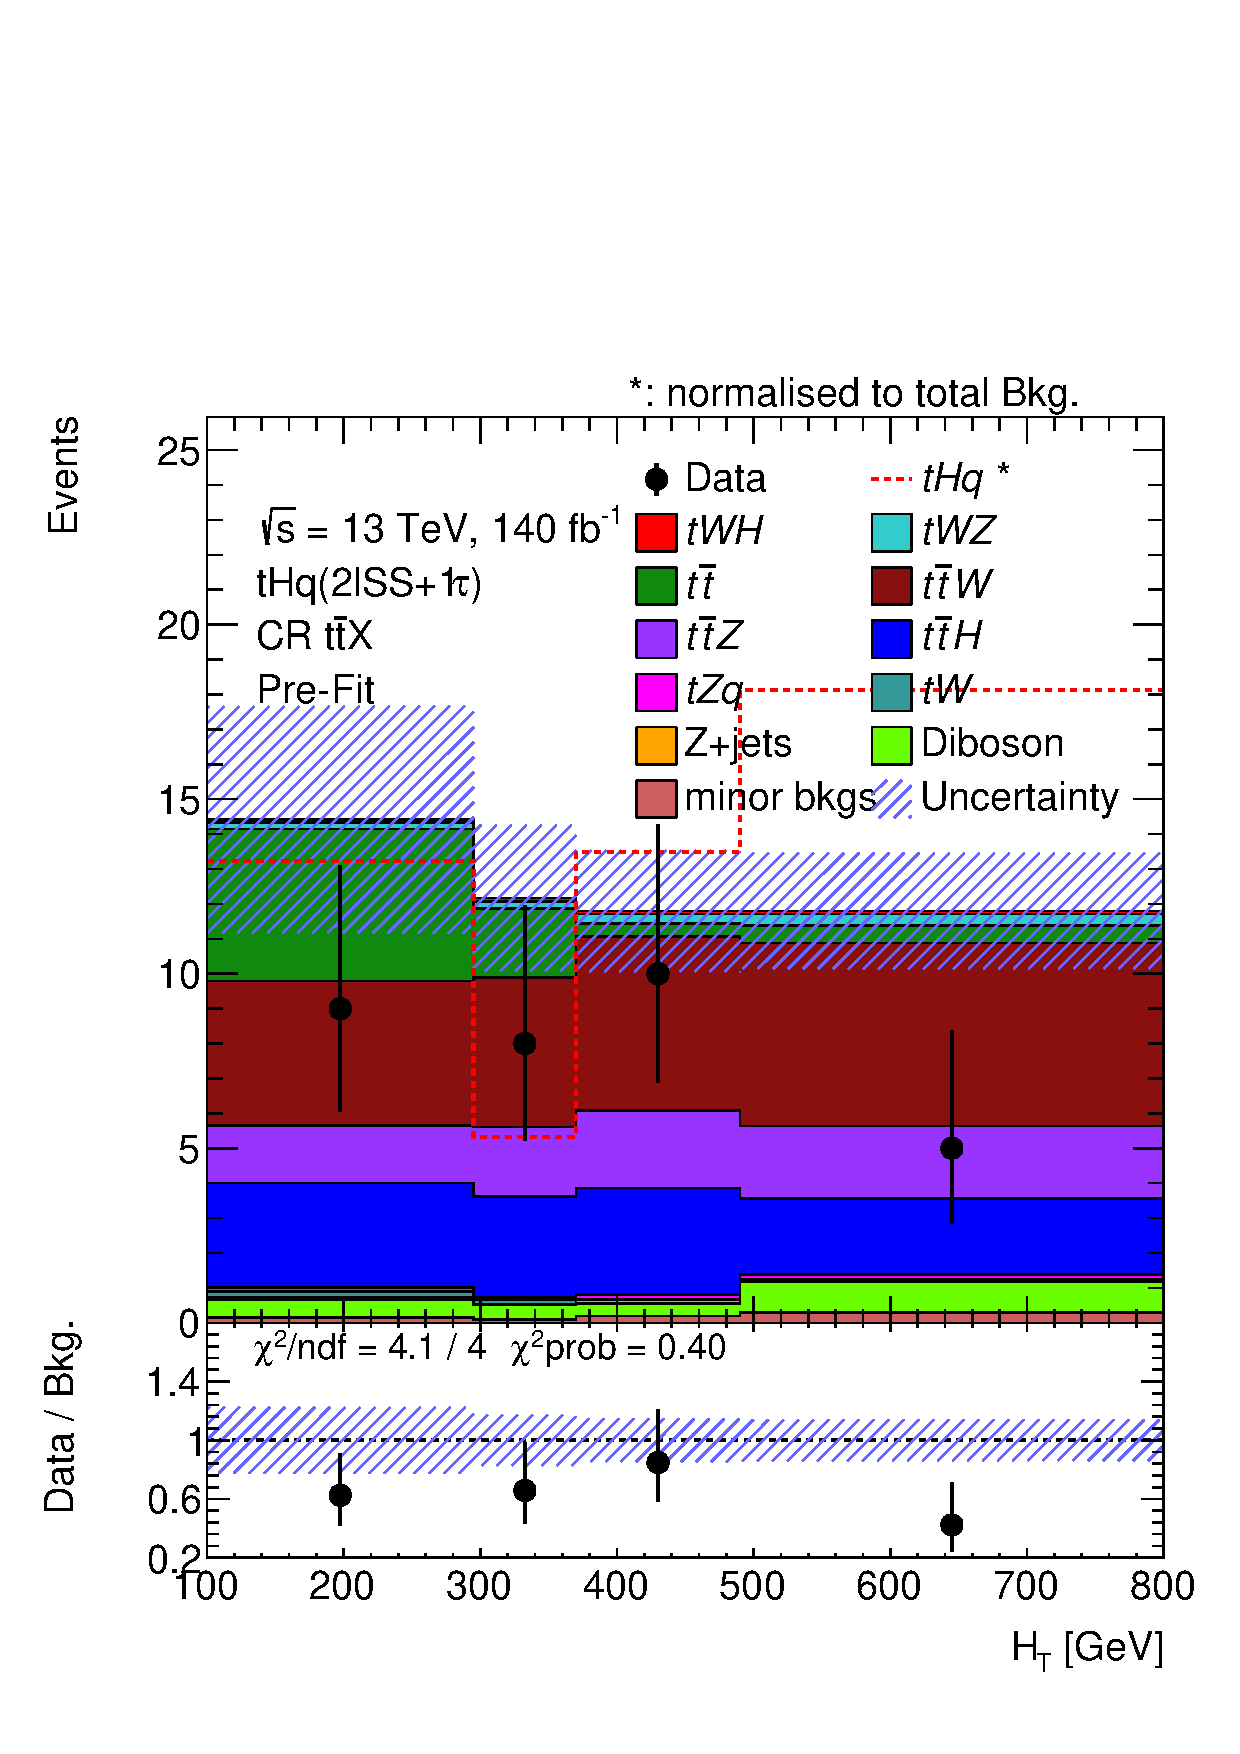
\includegraphics[width=.95\linewidth]{Chapter5_tHq/Alternative_Fit_Models/SS_CR-all_kttW/Asimov/CR_HT_2L1TAU_SS}
  \caption{$H_{\text{T}}$ is used for the CR(all bkgs).}
  \label{fig:Alternative:SS:OneCR_kttW:distributions:HT}
\end{subfigure}
\caption{Distributions used for the SR(\tHq) and CR(all bkgs) fit in \dilepSStau. 
	Note that the data is blinded in the SR.
	Observe the large discrepancy between data and the MC-simulated events.} % since we are under the Asimov hypothesis, the data/MC agreement is perfect in the SR
\label{fig:Alternative:SS:OneCR_kttW:distributions}
\end{figure}

The results of the fit using this configuration are presented in Table~\ref{tab:Alternative:SS:OneCR_kttW:results}.
The $k_{\ttW}$ factor obtained diverges significatively from one. This is not surprising since, as it is shown
in Figure~\ref{fig:Alternative:SS:OneCR_kttW:distributions:HT}, there is a large excess of MC over the data. 
Therefore, to correct this effect, the backgrounds have to be scaled by a factor smaller than one. 


\begin{table}[h]
\centering
\begin{tabular}{l|c|c}
\cline{2-3}
            		%& \multicolumn{2}{c}{$\mu_{\tHq}$} \\ \cline{2-3}
            		&   Asimov								&  \texttt{CRSR--background-only}       			\\ \midrule
$\mu_{\tHq}$ 	&  $\pm 6.74\text{(tot.)} \pm 5.76\text{(stat.)}$)        	&        -        \\
$k_{\ttW}$ 	&  $\pm 0.29\text{(tot.)} \pm 0.5\text{(stat.)}$)		&  $0.09\pm 0.39\text{(tot.)} \pm 0.22\text{(stat.)}$)        \\ \bottomrule
\end{tabular}
\caption{Values for $\mu_{\tHq}$ and $k_{\ttW}$ when fitting in the CR(all bkgs) only. 
Note that in the Asimov fit only the expected uncertainty is given. Also, note that in the \texttt{CRSR--background-only} fit the signal strength is not fitted.
This is explained in Section~\ref{sec:ChaptH:Fit:strategy}.}
\label{tab:Alternative:SS:OneCR_kttW:results}
\end{table}

Regarding the constraints and pulls, only a JES-related uncertainty presents constraints in the Asimov fit 
and pulls in the \texttt{CRSR--background-only}, the \texttt{JES effective NP stat. 6}.
\begin{figure}[h]
  \centering
  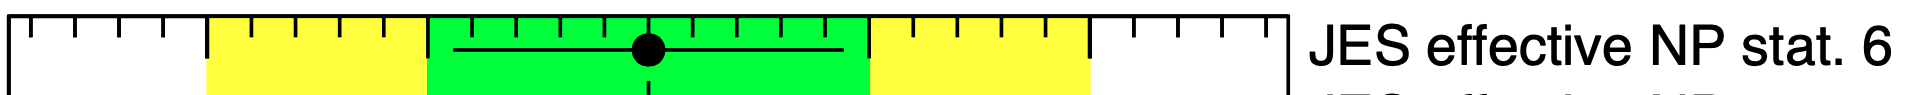
\includegraphics[width=.5\linewidth]{Chapter5_tHq/Alternative_Fit_Models/SS_CR-all_kttW/Asimov/Constaint}
  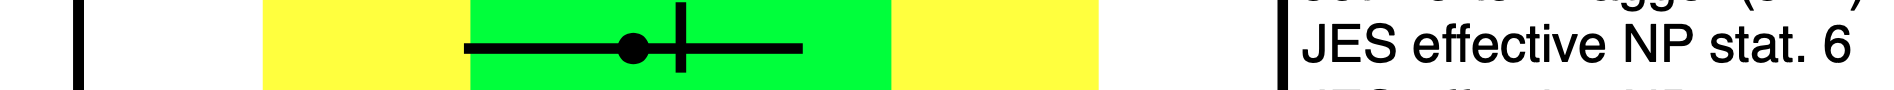
\includegraphics[width=.55\linewidth]{Chapter5_tHq/Alternative_Fit_Models/SS_CR-all_kttW/CRSR_bonly/pullA}
\caption{Constraint and pull of the  \texttt{JES effective NP stat. 6}.}
\label{fig:Alternative:SS:OneCR_kttW:pull}
\end{figure}


The correlation matrices for this fit are presented on Figure~\ref{fig:Alternative:SS:OneCR_kttW:matrices}, 
where it can be seen that the systematic uncertainty associated with the normalisation of the misidentified
\tauhad is highly anticorrelated with the $k_{\ttW}$. 
One of the JES uncertainties is also presenting an anticorrelation with the  signal strength. This particular
uncertainty is the only one that is constraint and pulled.  
The ranking plot is presented in Figure~\ref{fig:Alternative:SS:OneCR_kttW:ranking}. 

\begin{figure}[h]
\centering
\begin{subfigure}{.5\textwidth}
  \centering
  \includegraphics[width=.95\linewidth]{Chapter5_tHq/Alternative_Fit_Models/SS_CR-all_kttW/Asimov/CorrMatrix}
  \caption{Asimov fit.}
\end{subfigure}%
\begin{subfigure}{.5\textwidth}
  \centering
  \includegraphics[width=.95\linewidth]{Chapter5_tHq/Alternative_Fit_Models/SS_CR-all_kttW/CRSR_bonly/CorrMatrix}
  \caption{\texttt{CRSR--background-only} fit.}
\end{subfigure}
\caption{Correlation matrices for the fit with SR(\tHq) and CR(all bkgs) fit in \dilepSStau where \ttW is the only floating background.
	In the \texttt{CRSR--background-only} the SR is not fitted and, hence, the correlations with $\mu_{\tHq}$ are not calculated. }
\label{fig:Alternative:SS:OneCR_kttW:matrices}
\end{figure}


\begin{figure}[h]
\centering
  \centering
  \includegraphics[width=.75\linewidth]{Chapter5_tHq/Alternative_Fit_Models/SS_CR-all_kttW/Asimov/Ranking_tH_NORM}
\caption{Ranking for the \dilepSStau using CR(all bkgs). Note that it has been obtained under the Asimov hypothesis.}
\label{fig:Alternative:SS:OneCR_kttW:ranking}
\end{figure}


\subsection{Three regions and floating $k_{\ttW}$ and $k_{\ttbar}$}
\label{sec:Alternative:SS:twoCRs_kttW_kttbar}
In the fit configuration presented in Section~\ref{sec:Alternative:SS:OneCR_kttW}, the normalisation
factor obtained for \ttW is extremely small. Instead of heavily scaling down a single background process,
if several $k$ factors are let to float as free parameters, the compensation of the MC excess over data
can be split among the fitted processes. To do so, two CRs are defined:
\begin{itemize}
	\item SR(\tHq) :: BDT$(\tHq|_{\text{SS}}) \leq 0.4$ and fitting the BDT$(\tHq|_{\text{SS}})$ distribution.
	\item CR(\ttbar) :: BDT$(\tHq|_{\text{SS}}) > 0.4$, $H_{\text{T}} <260$~GeV and only one \btagged jet. Fitting $H_{\text{T}}$ distribution. 
	\item CR(\ttX) :: BDT$(\tHq|_{\text{SS}}) > 0.4$ and $H_{\text{T}} >260$~GeV.  Fitting $H_{\text{T}}$ distribution.
\end{itemize}
The distributions used for the fit are presented in Figure~\ref{fig:Alternative:SS:twoCRs_kttW_kttbar:Distributions}.

\begin{figure}[h]
  \centering  
  \begin{subfigure}[b]{0.49\textwidth}
    \centering
    \includegraphics[width=\textwidth]{Chapter5_tHq/Alternative_Fit_Models/SS_CR-tt_CR-ttX_ktt_kttW/CRSR_bonly/SR_BDT_tHq_2L1TAU_SS}
    \caption{BDT$(\tHq|_{\text{SS}})$ in SR(\tHq).}
     \label{fig:ChaptH:Alternative:SS:twoCRs_kttW_kttbar:Distributions:thq}
  \end{subfigure}
  \hfill
  \begin{subfigure}[b]{0.49\textwidth}
    \centering
    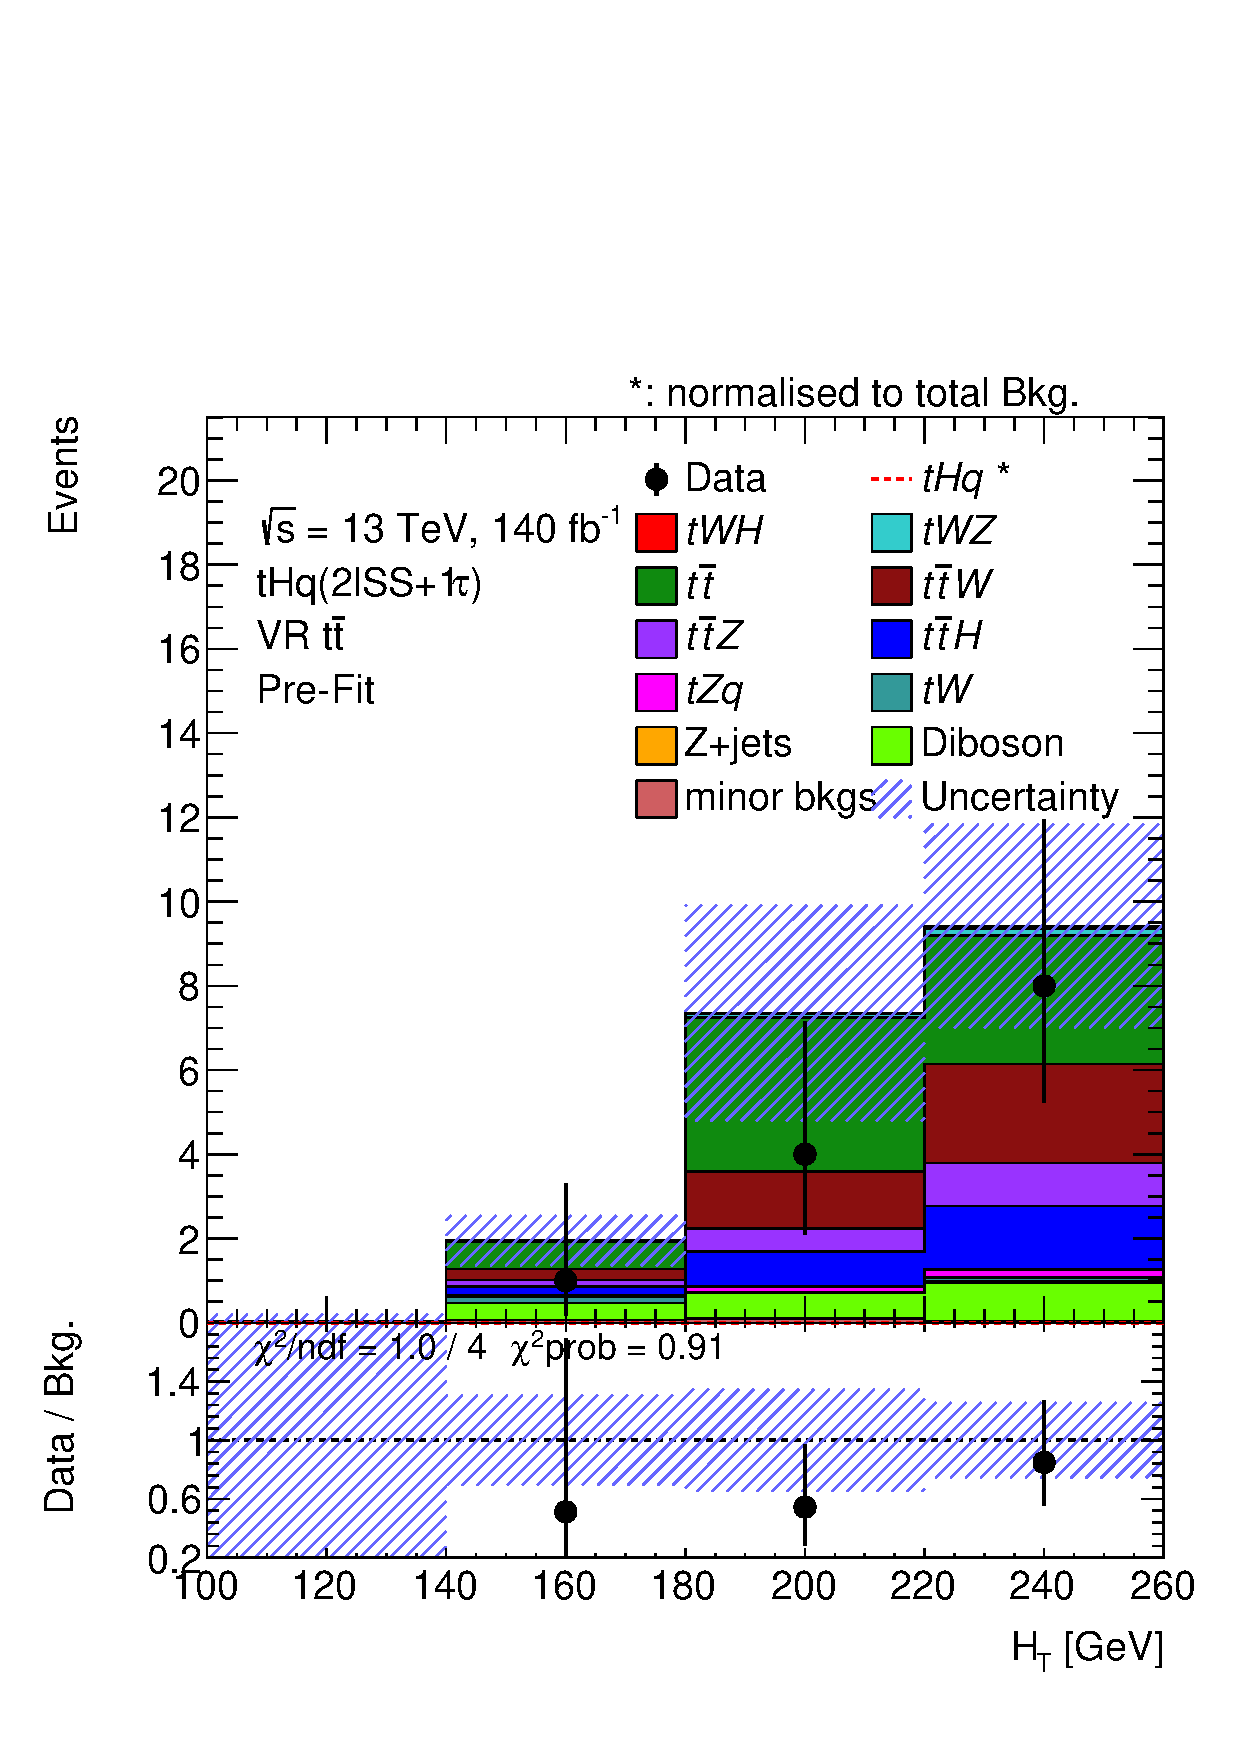
\includegraphics[width=\textwidth]{Chapter5_tHq/Alternative_Fit_Models/SS_CR-tt_CR-ttX_ktt_kttW/CRSR_bonly/CR_ttbar_2L1TAU_SS}
    \caption{$H_{\text{T}}$ in CR(\ttbar).}
     \label{fig:Alternative:SS:twoCRs_kttW_kttbar:Distributions:ttbar}
  \end{subfigure}
    \hfill
  \begin{subfigure}[b]{0.49\textwidth}
    \centering
    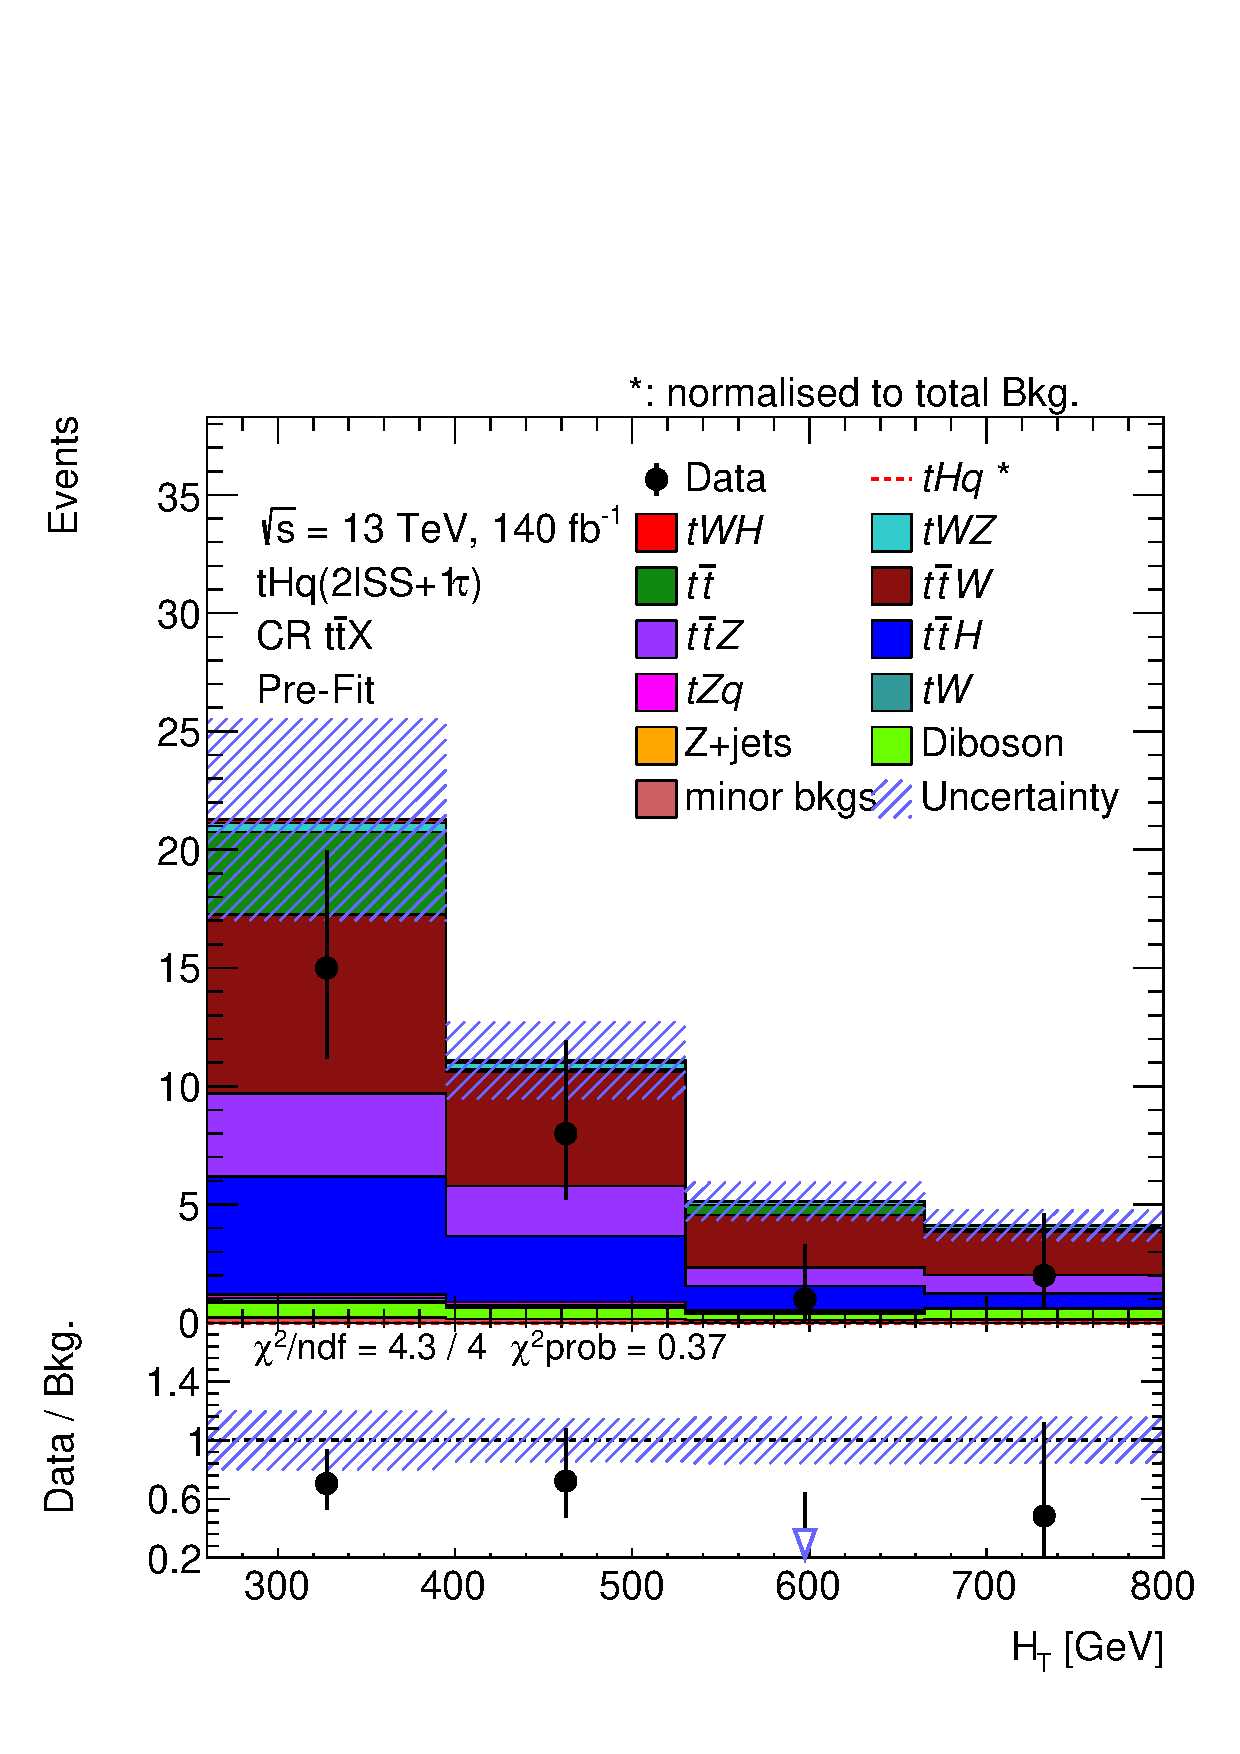
\includegraphics[width=\textwidth]{Chapter5_tHq/Alternative_Fit_Models/SS_CR-tt_CR-ttX_ktt_kttW/CRSR_bonly/CR_ttX_2L1TAU_SS}
    \caption{$H_{\text{T}}$ in CR(\ttX).}
     \label{fig:Alternative:SS:twoCRs_kttW_kttbar:Distributions:ttX}
  \end{subfigure}
  \caption{Distributions used for the \dilepSStau fit with two CRs and two $k$ factors. Note the first bin the the distribution for CR(\ttbar) has no events 
  and this may lead to instabilities in the fit.} 
  \label{fig:Alternative:SS:twoCRs_kttW_kttbar:Distributions}
\end{figure}

The results of the fit with two CRs and two $k$ factors is presented in Table~\ref{tab:Alternative:SS:twoCRs_kttW_kttbar:results}.
As can be seen, the compensation of the data/MC discrepancies has a larger impact in $k_{\ttW}$ than in $k_{\ttbar}$.
Alternatively, two other fits has been explored: 
\begin{itemize}
	\item The $k(\ttX)$ has been fitted instead of $k(\ttW)$. 
	\item The $k(\ttX + \ttbar)$ has been fitted instead of $k(\ttW)$ and $k(\ttbar)$. 
\end{itemize}
Non of these approaches yielded good results but the one using $k(\ttX)$ has bee
repeated in Section~\ref{sec:Alternative:SS:twoCRs_kttW_kttbar_Fixed}.

\begin{table}[h]
\centering
\begin{tabular}{l|c|c}
\cline{2-3}
            		%& \multicolumn{2}{c}{$\mu_{\tHq}$} \\ \cline{2-3}
            		&   Asimov								&  \texttt{CRSR--background-only}       			\\ \midrule
$\mu_{\tHq}$ 	&  $\pm 7.3\text{(tot.)} \pm 6.62\text{(stat.)}$)        	&        -        \\
$k_{\ttbar}$	&  $\pm 0.90\text{(tot.)} \pm 0.64\text{(stat.)}$) 		&  $0.65\pm 0.63\text{(tot.)} \pm 0.47\text{(stat.)}$)  \\
$k_{\ttW}$ 	&  $\pm 0.56\text{(tot.)} \pm 0.41\text{(stat.)}$)		&  $0.12\pm 0.43\text{(tot.)} \pm 0.33\text{(stat.)}$)        \\ \bottomrule
\end{tabular}
\caption{Values for $\mu_{\tHq}$, $k_{\ttbar}$, and $k_{\ttW}$.}
\label{tab:Alternative:SS:twoCRs_kttW_kttbar:results} 
\end{table}



\begin{figure}[h]
\centering
\begin{subfigure}{.5\textwidth}
  \centering
  \includegraphics[width=.95\linewidth]{Chapter5_tHq/Alternative_Fit_Models/SS_CR-tt_CR-ttX_ktt_kttW/Asimov/CorrMatrix}
  \caption{Asimov fit.}
\end{subfigure}%
\begin{subfigure}{.5\textwidth}
  \centering
  \includegraphics[width=.95\linewidth]{Chapter5_tHq/Alternative_Fit_Models/SS_CR-tt_CR-ttX_ktt_kttW/CRSR_bonly/CorrMatrix}
  \caption{\texttt{CRSR--background-only} fit.}
\end{subfigure}
\caption{Correlation matrices for \dilepSStau fit where the $k$ factors of \ttbar and \ttW are allowed to float as  free parameters of the fit.}
\label{fig:Alternative:SS:twoCRs_kttW_kttbar:matrices}
\end{figure}


\FloatBarrier

\subsection{Three regions and floating $k_{\ttX}$ and $k_{\ttbar}$ with fix}
\label{sec:Alternative:SS:twoCRs_kttW_kttbar_Fixed}
Here a quite similar fit as in the previous Section~\ref{sec:Alternative:SS:twoCRs_kttW_kttbar} is presented but
instead of floating \ttW, the entire \ttX is allowed to float. Additionally,  
the first bin of Figure~\ref{fig:Alternative:SS:twoCRs_kttW_kttbar:Distributions:ttbar} has been excluded from 
the calculations as can be seen in Figure~\ref{fig:Alternative:SS:twoCRs_kttX_kttbar_fixed:Distribution} because
it did not had any statistics and lead to inestabilities on the fit.
\begin{figure}[h!]
  \centering  
    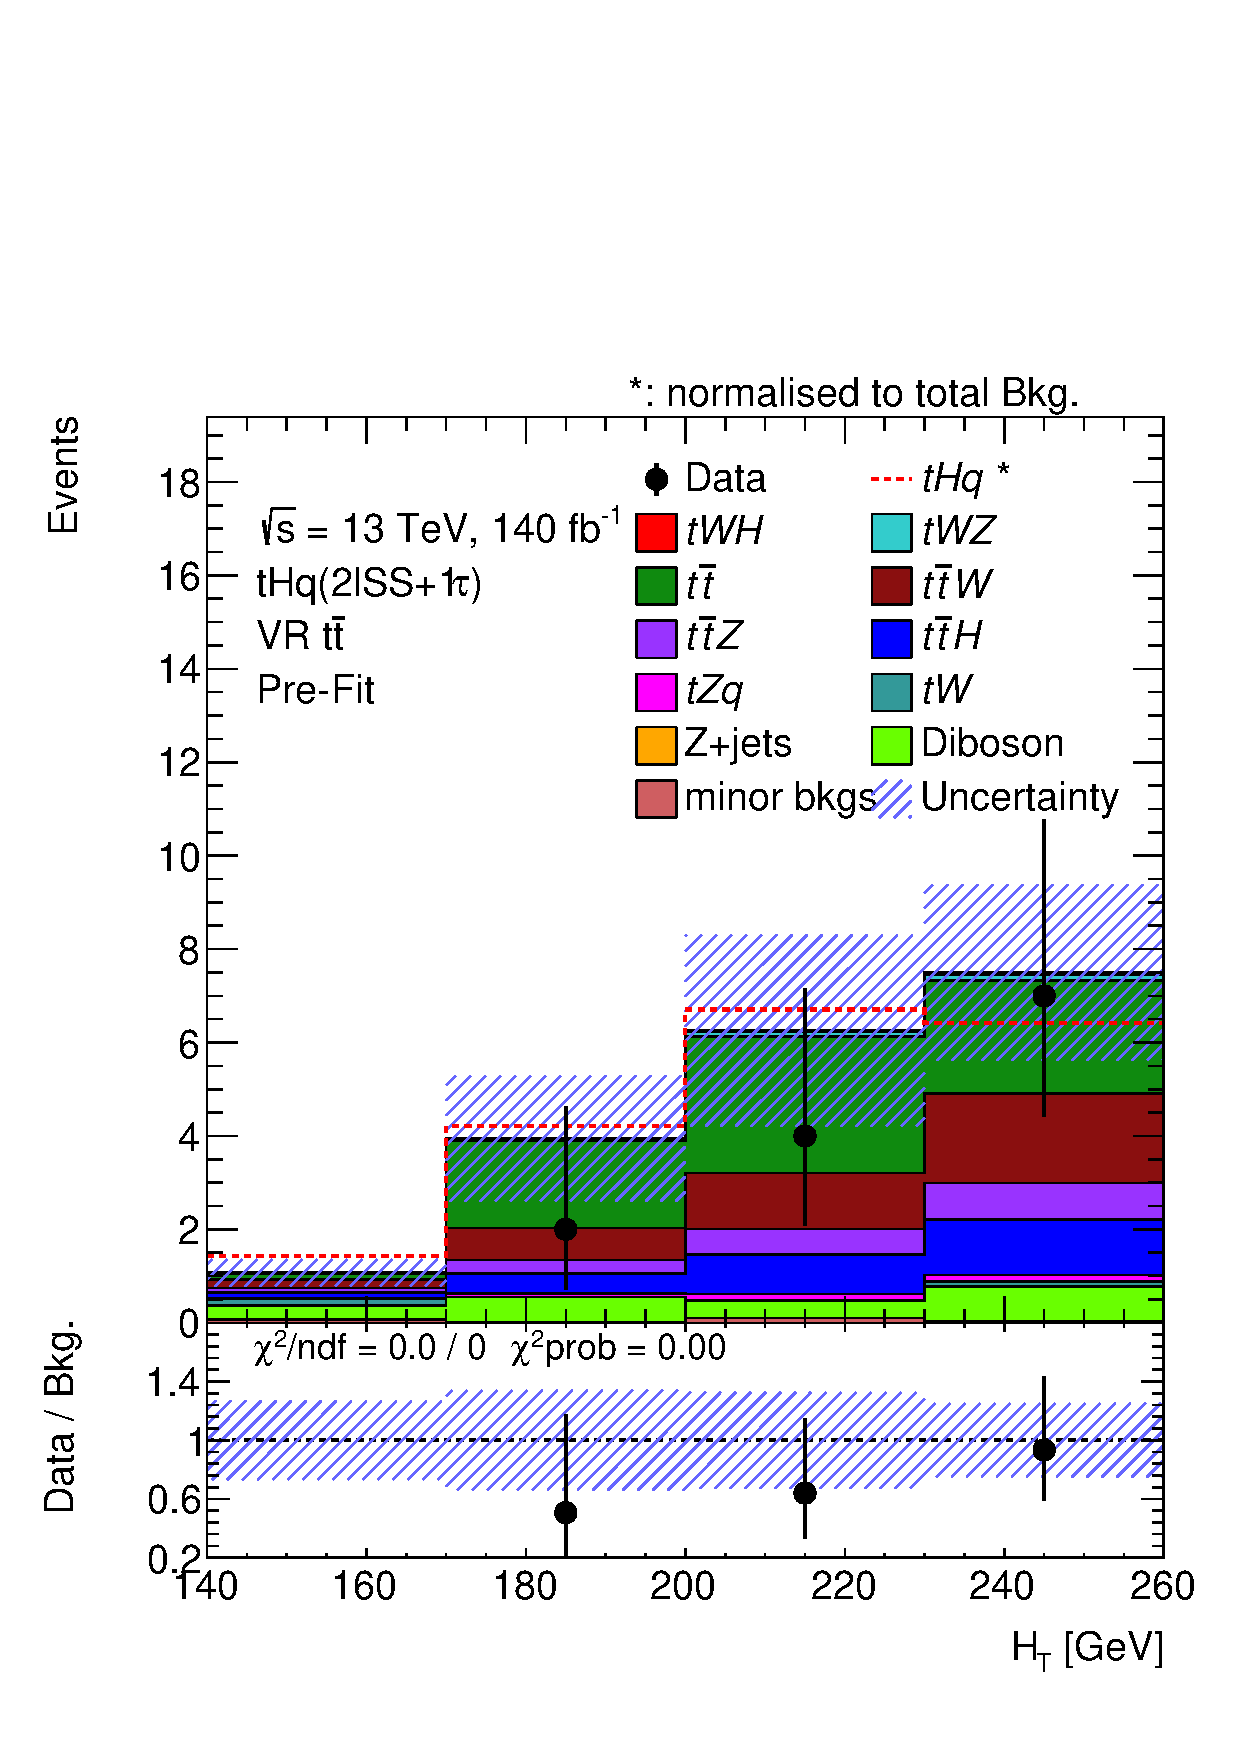
\includegraphics[width=0.45\textwidth]{Chapter5_tHq/Alternative_Fit_Models/SS_CR-tt_CR-ttX_ktt_kttX_Fix/asimov_dist_CR_ttbar_2L1TAU_SS}
  \caption{$H_{\text{T}}$ in CR(\ttbar).} 
  \label{fig:Alternative:SS:twoCRs_kttX_kttbar_fixed:Distribution}
\end{figure}
 
The gammas are contained in $1.0 \pm0.3$ as Figure~\ref{fig:Alternative:SS:twoCRs_kttX_kttbar_fixed:gammas}.
Within the Asimov hypothesis, the only constrained NP corresponds to the \ttbar NLO generator and no pulls are present in the \texttt{CRSR--background-only} fit.

\begin{figure}[h]
\centering
\begin{subfigure}{.35\textwidth}
  \centering
  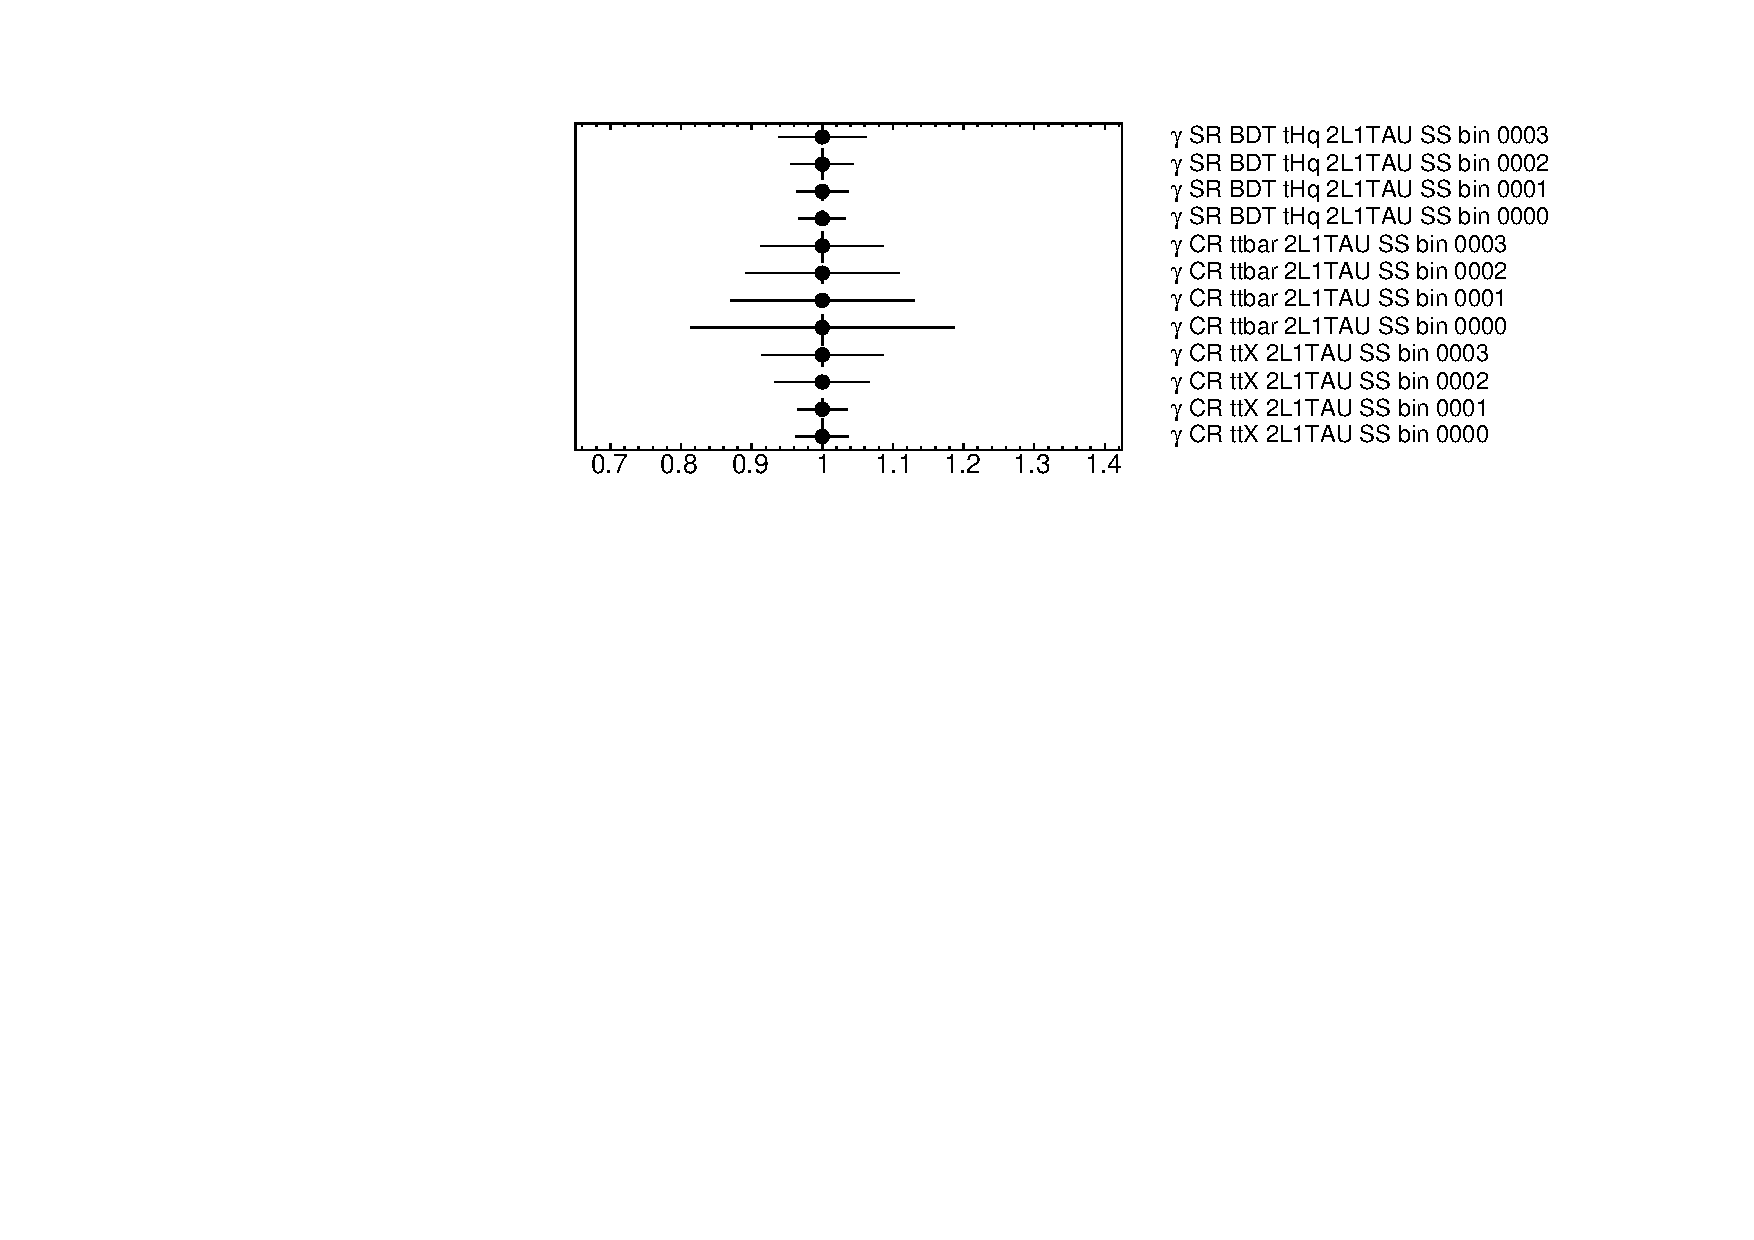
\includegraphics[width=.95\linewidth]{Chapter5_tHq/Alternative_Fit_Models/SS_CR-tt_CR-ttX_ktt_kttX_Fix/asimov_Gammas}
  \caption{Asimov fit.}
\end{subfigure}%2
\begin{subfigure}{.35\textwidth}
  \centering
  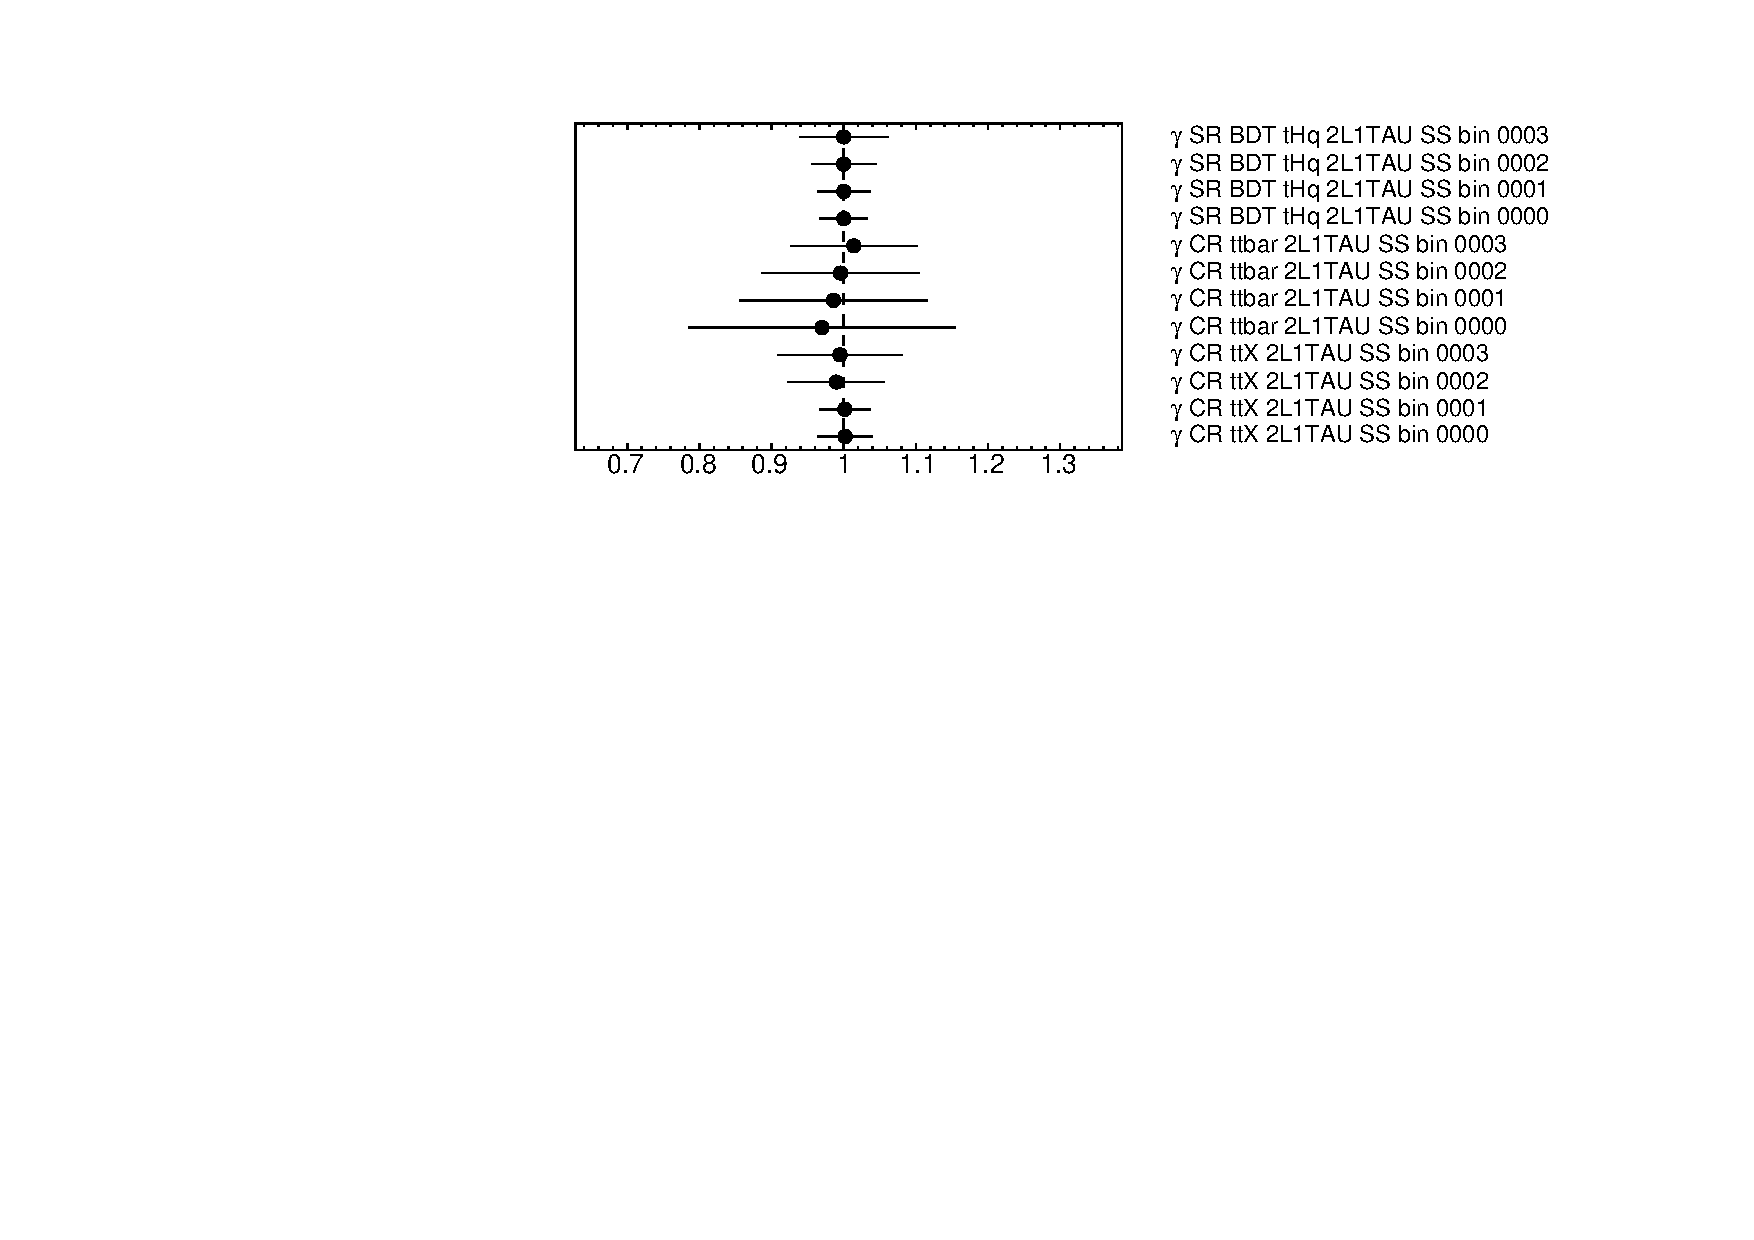
\includegraphics[width=.95\linewidth]{Chapter5_tHq/Alternative_Fit_Models/SS_CR-tt_CR-ttX_ktt_kttX_Fix/BONLY_CRSR_Gammas}
  \caption{\texttt{CRSR--background-only} fit.}
\end{subfigure}
\caption{Gramma plots}
\label{fig:Alternative:SS:twoCRs_kttX_kttbar_fixed:gammas}
\end{figure}

The signal strength and normalisation factors of \ttbar and \ttX under this fit configuration are 
presented in Table~\ref{tab:Alternative:SS:twoCRs_kttX_kttbar_fixed:results}. 

\begin{table}[h]
\centering
\begin{tabular}{l|c|c}
\cline{2-3}
            		%& \multicolumn{2}{c}{$\mu_{\tHq}$} \\ \cline{2-3}
            		&   Asimov								&  \texttt{CRSR--background-only}       			\\ \midrule
$\mu_{\tHq}$ 	&  $\pm 7.25\text{(tot.)} \pm 6.59\text{(stat.)}$)        	&        -        \\
$k_{\ttbar}$	&  $\pm 0.92\text{(tot.)} \pm 0.66\text{(stat.)}$) 		&  $0.75\pm 0.68\text{(tot.)} \pm 0.50\text{(stat.)}$)  \\
$k_{\ttX}$ 		&  $\pm 0.28\text{(tot.)} \pm 0.20\text{(stat.)}$)		&  $0.57\pm 0.21\text{(tot.)} \pm 0.17\text{(stat.)}$)        \\ \bottomrule
\end{tabular}
\caption{Values for $\mu_{\tHq}$, $k_{\ttbar}$, and $k_{\ttW}$.}
\label{tab:Alternative:SS:twoCRs_kttX_kttbar_fixed:results} 
\end{table}





